\section{FreeCAD}
FreeCAD is a general purpose parametric 3D CAD modeler. The development 
is completely Open Source (LGPL License). FreeCAD is aimed directly at  
mechanical engineering and product design but also fits in a wider range
of uses around engineering, such as architecture or other engineering specialties.
                                                                        
FreeCAD features tools similar to Catia, SolidWorks or Solid Edge, and  
therefore also falls into the category of MCAD, PLM, CAx and CAE. It is a
feature based parametric modeler with a modular software architecture which
makes it easy to provide additional functionality without modifying the core system.
                                                                        
As with many modern 3D CAD modelers it has many 2D components in order  
to sketch 2D shapes or extract design details from the 3D model to create
2D production drawings, but direct 2D drawing (like AutoCAD LT) is not the
focus, neither are animation or organic shapes (like Maya, 3ds Max, Blender
or Cinema 4D), although, thanks to its wide adaptability, FreeCAD might 
become useful in a much broader area than its current focus.            
                                                                        
FreeCAD makes heavy use of all the great open-source libraries that exist
out there in the field of Scientific Computing. Among them are OpenCascade,
a powerful CAD kernel, Coin3D, an incarnation of Open Inventor, Qt, the world-famous
UI framework, and Python, one of the best scripting languages available.
FreeCAD itself can also be used as a library by other programs.         
                                                                        
FreeCAD is also fully multi-platform, and currently runs flawlessly on  
Windows and Linux/Unix and Mac OSX systems, with the exact same look and
functionality on all platforms.

\subsection{FreeCAD's features}
\subsubsection{Key features}
\begin{itemize}
\item A complete Open CASCADE Technology-based geometry kernel allowing 
complex 3D operations on complex shape types, with native support for 
concepts like brep, nurbs curves and surfaces, a wide range of geometric 
entities, boolean operations and fillets, and built-in support of STEP and 
IGES formats.
\item A full parametric model. All FreeCAD objects are natively parametric, 
which means their shape can be based on properties or even depend on other 
objects, all changes being recalculated on demand, and recorded by the 
undo/redo stack. New object types can be added easily, that can even be 
fully programmed in Python.
\item A modular architecture that allow plugins (modules) to add functionality
to the core application. Those extensions can be as complex as whole new
applications programmed in C++ or as simple as Python scripts or self-recorded
macros. You have complete access from the Python built-in interpreter,
macros or external scripts to almost any part of FreeCAD, being geometry 
creation and transformation, the 2D or 3D representation of that geometry 
(scenegraph) or even the FreeCAD interface.
\item Import/export to standard formats such as STEP, IGES, OBJ, STL, DXF, 
SVG, STL, DAE, IFC or OFF, NASTRAN, VRML in addition to FreeCAD's native 
Fcstd file format. The level of compatibility between FreeCAD and a given 
file format can vary, since it depends on the module that implements it.
\item A Sketcher with constraint-solver, allowing to sketch geometry-constrained 
2D shapes. The sketcher currently allows you to build several types of 
constrained geomerty, and use them as a base to build other objects throughout 
FreeCAD.
\item A Robot simulation module that allows to study robot movements. The 
robot module already has an extended graphical interface allowing GUI-only 
workflow.
\item A Drawing sheets module that permit to put 2D views of your 3D 
models on a sheet. This modules then produces ready-to-export SVG or PDF 
sheets. The module is still sparse but already features a powerful Python 
functionality.
\item A Rendering module that can export 3D objects for rendering with 
external renderers. Currently only supports povray and LuxRender, but is 
expected to be extended to other renderers in the future.
\item An Architecture module that allows BIM-like workflow, with IFC 
compatibility. The making of the Arch module is heavily discussed by the 
community here.
\end{itemize}


\subsection{FreeCAD workbenches used in this project}
\subsection{Part module}
The CAD capabilities of FreeCAD are based on the OpenCasCade kernel. The 
Part module allows FreeCAD to access and use the OpenCasCade objects and 
functions. OpenCascade is a professional-level CAD kernel, that features 
advanced 3D geometry manipulation and objects. The Part objects, unlike 
Mesh Module objects, are much more complex, and therefore permit much more 
advanced operations, like coherent boolean operations, modifications history 
and parametric behaviour.
\begin{figure}[h!]                                                       
\begin{center}                                                          
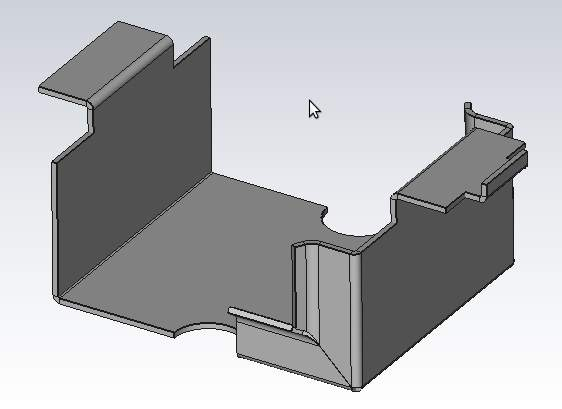
\includegraphics[scale=0.5]{images/Part_example.jpg}                     
\caption{Example of Part shapes in FreeCAD}                             \end{center} 
\end{figure}
\subsubsection{Draft module}
The Draft workbench allows to quickly draw simple 2D objects in the current 
document, and offers several tools to modify them afterwards. Some of these 
tools also work on all other FreeCAD objects, not only those created with 
the Draft workbench. It also provides a complete snapping system, and 
several utilities to manage objects and settings.
\subsection{Drawing module}
The Drawing module allows you to put your 3D work on paper. That is, to 
put views of your models in a 2D window and to insert that window in a drawing, 
for example a sheet with a border, a title and your logo and finally print that 
sheet. The Drawing module is currently under construction and more or less 
a technology preview!
\begin{figure}[h!]                                                       
\begin{center}                                                          
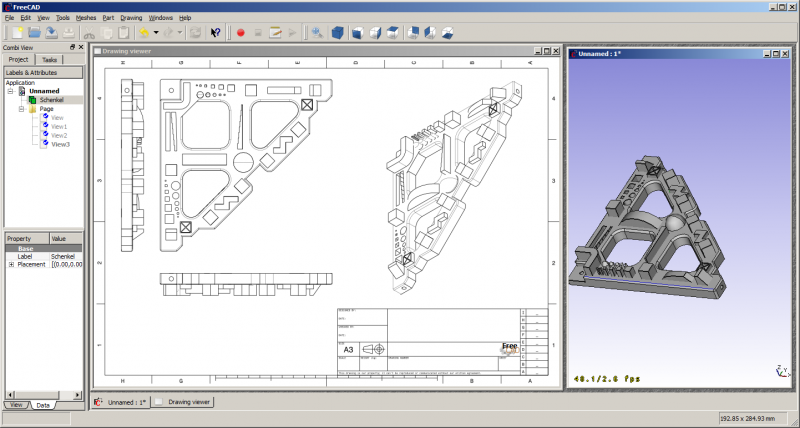
\includegraphics[scale=0.5]{images/Drawing_extraction.png}                     
\caption{Example of Drawing module in FreeCAD}                           \end{center}
\end{figure}

\subsection{Design implementation using Python scripting language}
Python is a programming language, very simple to use and very fast to learn. 
It is open-source, multi-platform, and can be used alone for a wide array of 
things, from programming simple shell scripts to very complex programs. But 
one of its most widespread uses is as a scripting language, since it is easy 
to embed in other applications. That's exactly how it is used inside FreeCAD. 
From the python console, or from your custom scripts, you can pilot FreeCAD, 
and make it perform very complex actions for which there is still no graphical 
user interface tool.\\
For example, from a python script, you can:
\begin{itemize}
\item create new objects
\item modify existing objects
\item modify the 3D representation of those objects
\item modify the FreeCAD interface
\end{itemize}
There are also several different ways to use python in FreeCAD:
\begin{itemize}
\item From the FreeCAD python interpreter, where you can issue simple commands like in a "command line"-style interface
\item From macros, which are a convenient way to quickly add a missing tool to the FreeCAD interface
\item From external scripts, which can be used to program much more complex things. like entire Workbenches.
\end{itemize}
\subsubsection{Writing python code}
There are two easy ways to write python code in FreeCAD: From the python 
console (available from the View -> Panels -> Python console menu) or from 
the Macro editor (Tools -> Macros). In the console, you write python commands 
one by one, which are executed when you press return, while the macros can 
contain a more complex script made of several lines, which is executed only 
when the macro is executed.
\begin{figure}[h!]                                                       
\begin{center}                                                          
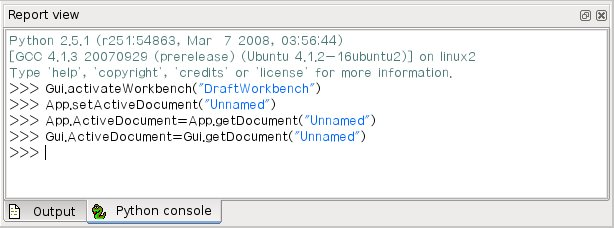
\includegraphics[scale=0.5]{images/Screenshot_pythoninterpreter.jpg}                     
\caption{Example of python scripting}
\end{center}
\end{figure} 

\subsection{Macros}
Macros are a convenient way to create complex actions in FreeCAD. You simply 
record actions as you do them, then save that under a name, and replay them 
whenever you want. Since macros are in reality a list of python commands, 
you can also edit them, and create very complex scripts.

In this project I have made many macros which are using for different purposes.
\begin{itemize}
\item \textbf{Builing macro:} This macro will create the model of building by
using the user input in 3D space of FreeCAD. For running this macro in the 
project I have used the below command.
\begin{verbatim}
freecadcmd builing_macro.py
\end{verbatim}
\begin{figure}[h!]                                                      
\begin{center}                                                          
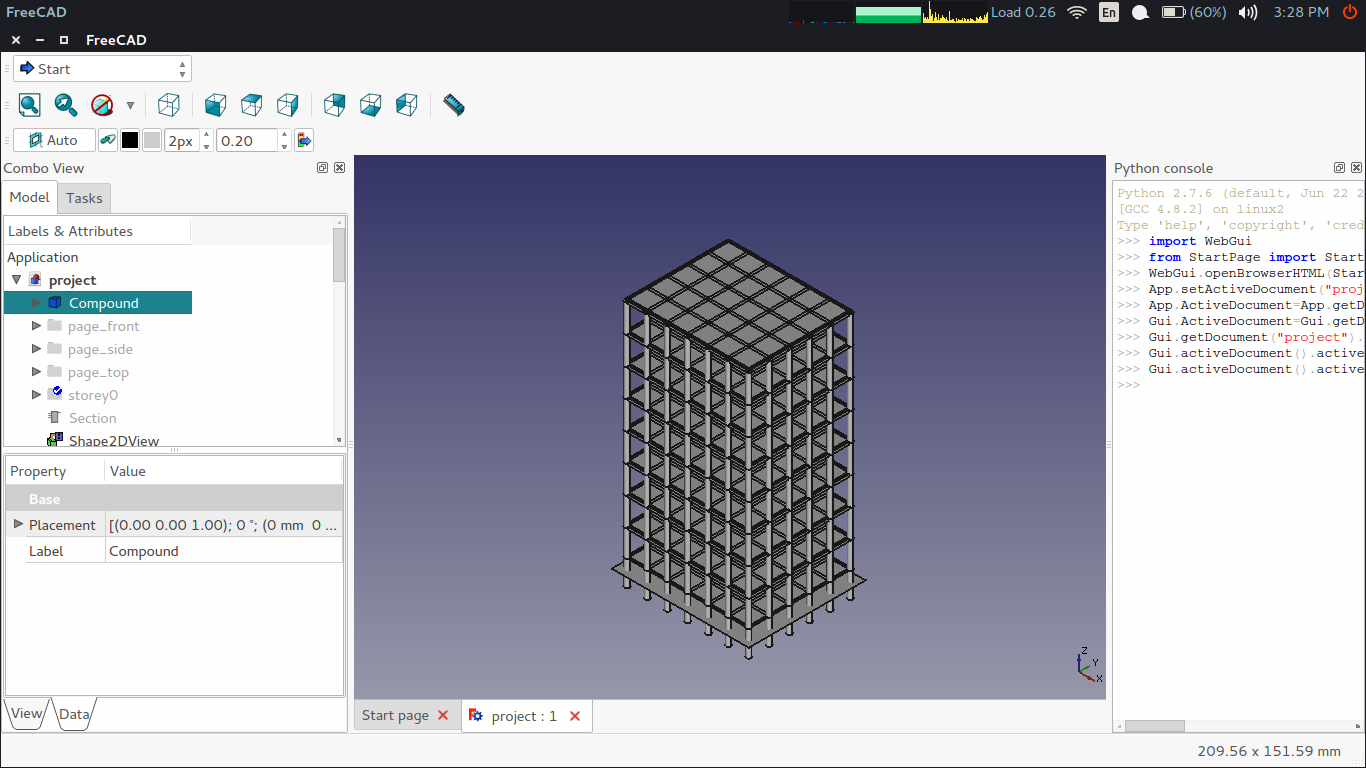
\includegraphics[scale=0.35]{images/building_macro.png}
\caption{Example of building macro}                                   
\end{center}                                                            
\end{figure}
\item \textbf{Drawing macro:} This macro will draw the drawing of different 
views (top, front and side view) of the builing along with sectional view of each 
building storey on the drawing sheet.
(3D model).
\begin{verbatim}                                                      
freecadcmd drawing.py                                                
\end{verbatim}
\begin{figure}[h!]                                                      
\begin{center}                                                          
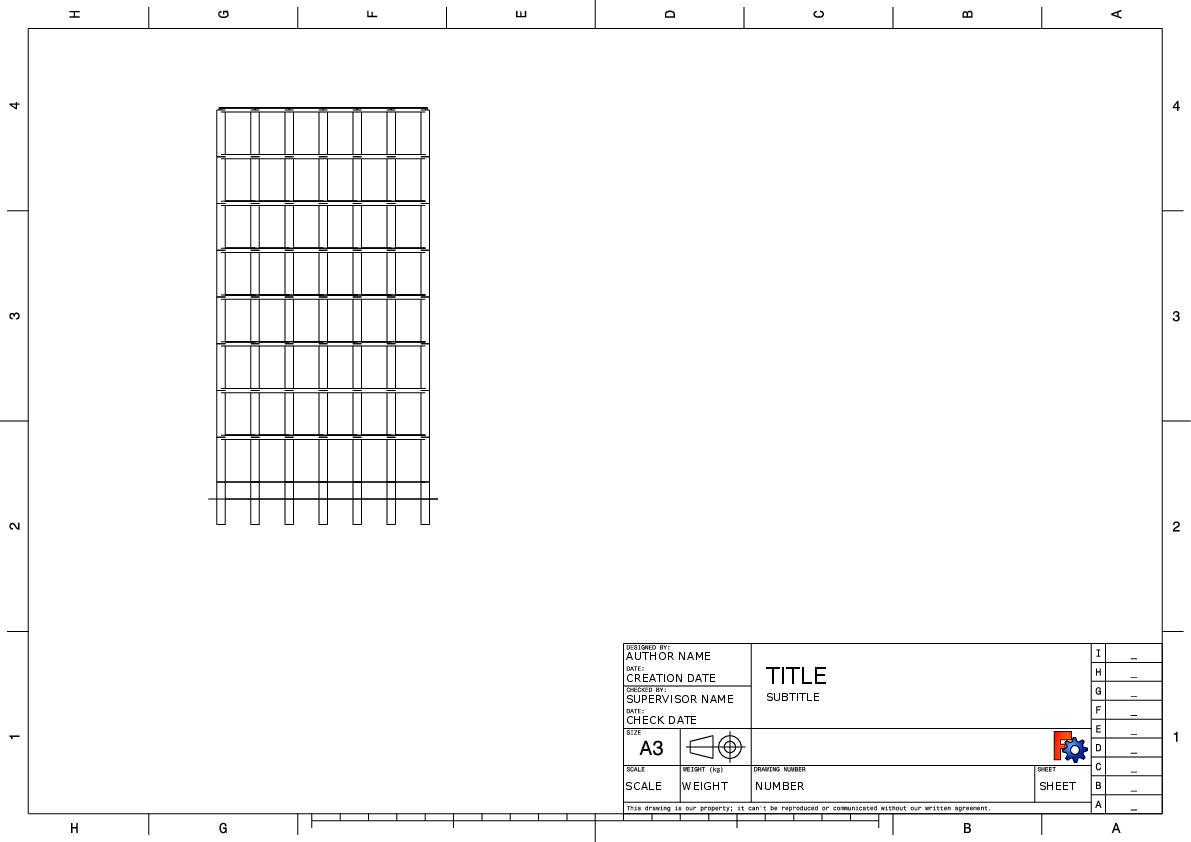
\includegraphics[scale=0.35]{images/page_side.png}
\caption{Example of drawing macro}                                   
\end{center}                                                            
\end{figure}
 
\item \textbf{Saving drawing macro:} This macro will save the drawing of the 
building in SVG (Scalable Vector Graphics) and then convert SVG file into PDF 
(Portable Document Format).
\begin{verbatim}                                                      
freecadcmd save_drawing.py                                                
\end{verbatim} 
\end{itemize}


\section{Inkscape}
Inkscape is an open source drawing tool for creating and editing SVG graphics. More than just a text vector
editor, Inkscape provides a WYSIWYG interface for manipulation of vector images, allowing the artist to
express himself freely. While other free and proprietary software exists with similar capabilities, Inkscape
provides an interface to directly manipulate the underlying SVG code, which allows one to be certain that the
code is in compliance with W3C standards. Since the beginning of its development, the Inkscape project has
been a very active, providing stability for the current software and growth of capacities in the future.
Like other drawing programs, Inkscape offers creation of basic shapes (such as ellipses, rectangles, stars,
polygons and spirals) as well as the ability to transform and manipulate these basic shapes by rotation,
stretching and skewing.

Inkscape also offers functionality to manipulate objects more precisely by adjusting node points and curves.
These functions are indispensable to useful drawing software, and allow the advanced artist to freely create
what he imagines.

The properties of objects can either be manipulated individually and precisely through the XML editor, or
more generally in an intuitive fashion by input devices such as mice, pen tablets or even touch screen.
In addition, Inkscape allows one to insert text and bitmaps (such as PNG, another W3C recommended bitmap
image format) into an image as well as perform some basic editing functions on them. If further bitmap
editing is required, other tools may be used (such as the GIMP) on images before importing them or after. In
fact, if a linked bitmap is edited in another program, Inkscape will reflect these changes once the SVG is
reloaded.

All of these characteristics make Inkscape a model drawing application, especially considering its flexibility
and many other capabilities. Its strict compliance with the W3C SVG standards allow excellent portability of
images to many applications and platforms on which these applications are used.

\subsection{About SVG}
Those who work with graphics for internet use are familiar with the problems tied to publication of images on
the web. Traditionally, bitmap images (such as JPG or GIF) have been the only option for use in such
documents, with the disadvantage that these images are either too large for quick transfer or, if they are small
or highly compressed to reduce file-size, of poor quality.

As a solution to this problem, Macromedia created the Flash image format. While Flash satisfactorily solved
the main problems inherent to bitmap images, there has been discontent for some users that the common
vector format for the web is dependent solely on Macromedia for development of the file format and
software. In order to address this discontent and provide an open option for vector graphics, the W3C created
the SVG file format, making a freely usable vector format available to everyone.

Most image files are only able to be read by specific software that renders the image. SVG, however, is
described in XML and CSS, and its files can be opened and edited in any ASCII text editor. While it is
possible to create SVG images in this manner, it is highly unproductive and unintuitive. SVG editors and
renderers have the ability to easily open and manipulate SVG files without a special interpreter.

\subsection{Objectives of the SVG Format}
The advantages of SVG are the same as for any vector image: high-quality images that are smooth and crisp
ability to resize the image to any dimensions without diminishing quality, which is impossible with bitmap
images. The SVG standard also defines animation, and with a little use of Javascript, one can make SVG
interactive. Finally, since SVG is written in XML, it is possible to create graphics based on data that is stored
in other XML-based formats, such as graphs, charts and maps. Despite its benefits, there is a lack of usable
software to create and edit SVG files and take full advantage of its capacities; for this reason, SVG is not as
usable at the moment as Flash.

\subsection{Export PDF macro}
It uses Inkscape to do the SVG to PDF conversion. Customize ToolsBar 
instructions can be used to add tool button in Drawing WB and therefore 
to be able to use Export PDF macro with ease when needed.
\begin{verbatim}  
import os
import subprocess
from PySide import QtGui

obj = FreeCADGui.Selection.getSelection()[0]

# Path to Inkscape executable
inkscape_path = "/usr/bin/inkscape"
# Exported PDF file location
file_location = os.path.expanduser("~" + os.sep + obj.Label + ".pdf")

# -------------------------------------------------------------------
try:
  page = getattr(obj, 'PageResult')
  except AttributeError:
    QtGui.QMessageBox.warning(None,"Export PDF", "Page object has \
        not been selected.")
    else:
        file_exists = os.path.isfile(file_location)
            if file_exists == True:
                QtGui.QMessageBox.warning(None,"Export PDF", "A \
                    file with the name " + obj.Label + ".pdf already \
                        exists:\n\n" + file_location)
                    else:
                         call_inkscape = [inkscape_path, "-f", \
                            obj.PageResult,"-A", file_location]
                         subprocess.call(call_inkscape)
                         QtGui.QMessageBox.information(None,"Export \
                            PDF", "Successfully exported:\n\n" + \
                                file_location)
\end{verbatim}  

\subsubsection{What does it do?}
It exports drawing page to PDF file using Inkscape. Instead of bitmap 
image inserted in PDF file elements like text are searchable and exported 
PDF file size can be smaller when the drawings do not have big number of 
elements in it.
\subsubsection{How to use it}
\begin{itemize}
\item Select Page object in Tree View.
\item Run Export PDF macro.
\end{itemize}

\section{C++}

\begin{figure}[h]
    \centering 
\includegraphics[scale=0.3]{images/c++.png}
    \caption{C++ Logo}
\end{figure}

C++ is a general-purpose programming language. It has imperative, object-oriented and generic programming features, while also providing facilities for low-level memory manipulation.

It was designed with a bias toward system programming and embedded, resource-constrained and large systems, with performance, efficiency and flexibility of use as its design highlights. C++ has also been found useful in many other contexts, with key strengths being software infrastructure and resource-constrained applications, including desktop applications, servers (e.g. e-commerce, web search or SQL servers), and performance-critical applications (e.g. telephone switches or space probes). C++ is a compiled language, with implementations of it available on many platforms and provided by various organizations, including the Free Software Foundation (FSF's GCC), LLVM, Microsoft, Intel and IBM.

C++ is standardized by the International Organization for Standardization (ISO), with the latest standard version ratified and published by ISO in December 2014 as ISO/IEC 14882:2014 (informally known as C++14). The C++ programming language was initially standardized in 1998 as ISO/IEC 14882:1998, which was then amended by the C++03, ISO/IEC 14882:2003, standard. The current C++14 standard supersedes these and C++11, with new features and an enlarged standard library. Before the initial standardization in 1998, C++ was developed by Bjarne Stroustrup at Bell Labs since 1979, as an extension of the C language as he wanted an efficient and flexible language similar to C, which also provided high-level features for program organization.

Many other programming languages have been influenced by C++, including C\#, D, Java, and newer versions of C (after 1998).

Features of Language:
\begin{enumerate}
    \item Object storage
    \begin{enumerate}
        \item Static storage duration objects
        \item Thread storage duration objects
        \item Automatic storage duration objects
        \item Dynamic storage duration objects
    \end{enumerate}
    \item Templates
    \item Objects
    \begin{enumerate}
        \item Encapsulation
        \item Inheritance
    \end{enumerate}
    \item Operators and operator overloading
    \item Polymorphism
    \begin{enumerate}
        \item Static polymorphism
        \item Dynamic polymorphism
        \begin{enumerate}
            \item Inheritance
            \item Virtual member functions
        \end{enumerate}
    \end{enumerate}
\item Lambda expressions
\item Exception handling
\end{enumerate}
